\section{Demografis indflydelse på vurderinger}
\label{sec:Demografi}
%
I dette afsnit beskrives hvordan forskellene mellem testpersonerne kan være med til at påvirke vurderingen af robotten. Der fokuseres isoleret på hvordan de demografiske faktorer påvirker hver enkelte skala. Det er valgt kun at medtage de grafer, hvor der forekommer en tendens for korrelation mellem alder og besvarelser til skalaerne. Dog er analysen foretaget på tværs af alle demografiske faktorer og samtlige skalaer, med undtagelse af hvor ofte testpersonerne rejser. Årsagen til at analysen ikke foretages i forhold til hvor ofte testpersonerne rejser skyldes hovedsageligt én ting, at AAL er relativt lille lufthavn, hvor der formentlig ikke er et lige så stort behov for robottens hjælp, som eksempelvis kan være tilfældet i Københavns Lufthavn. Med det i betragtning antages det, at for rejsende, som rejser privat flere gange årligt eller som rejser i forbindelse med arbejde, formentlig ikke adskiller sig specielt meget. Hvorimod hvis undersøgelsen blev foretaget i en større lufthavn, så kan det sagtens være at der er en forskel. Dette kan formentlig have særlig betydning for testpersonernes vurdering i forhold til hvorvidt de føler, at robotten kan hjælpe dem, om de stoler på, at den følger dem det rigtige sted hen, om den står i vejen og hvorvidt robotten opleves som værende anmassende.\blankline
% 
I henhold til testpersonernes alder tyder det på, at der er en positiv korrelation mellem alder og SQ6, jævnfør \autoref{fig:AgeSQ6}. Der er derfor en tendens til at desto ældre testpersonerne er, desto mere synes de, at robotten kører for hurtigt. 
%
\begin{figure}[H]
\centering
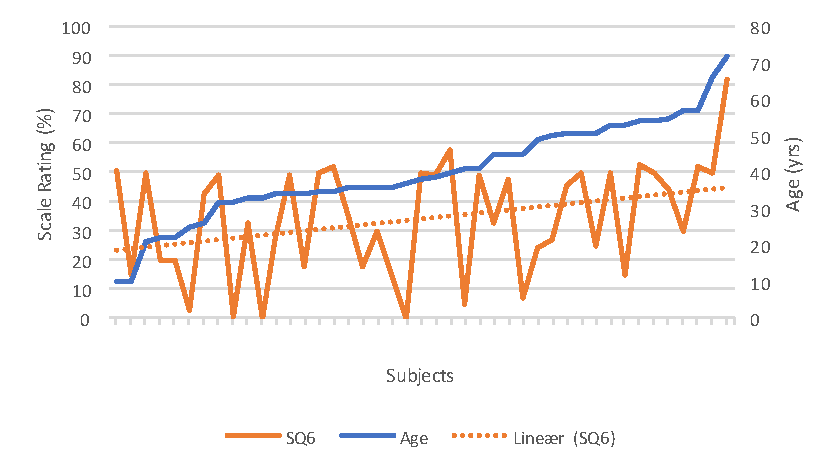
\includegraphics[width=\textwidth]{Figure/DatabehandlingSkalaer/Demografi/AgeSQ6}
\caption{Sammenhæng mellem hvad testpersonerne angiver (\%) på skalaen til SQ6: \textit{Jeg synes, at robottens hastighed er...}, og deres alder. Denne graf bygger på samtlige besvarelser.}
\label{fig:AgeSQ6}
\end{figure}
\noindent
%
Derudover forekommer der en lille negativ korrelation mellem testpersonernes alder og hvor spændende de synes robotten er, jævnfør \autoref{fig:AgeSQ18}. Der er derfor en tendens til at desto ældre testpersonerne, desto mindre spændende synes de, at robotten er. Derudover tyder det på at testpersoner mellem 35 år og 45 år finder robotten mindst spændende.
%
\begin{figure}[H]
\centering
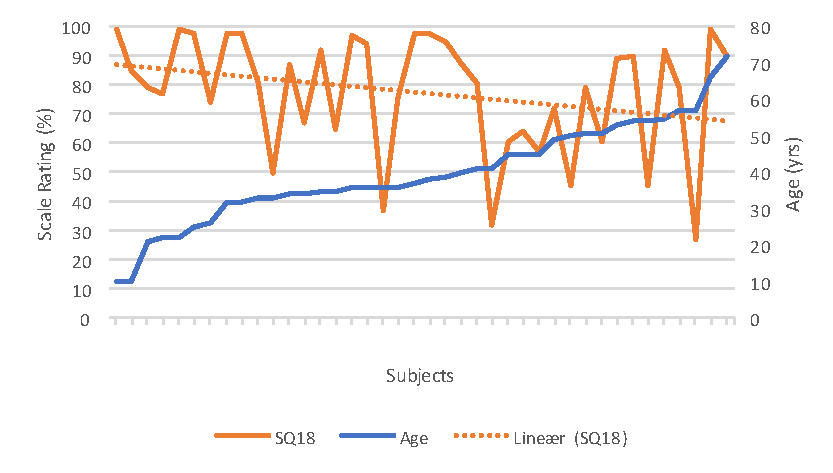
\includegraphics[width=\textwidth]{Figure/DatabehandlingSkalaer/Demografi/AgeSQ18}
\caption{Sammenhæng mellem hvad testpersonerne angiver (\%) på skalaen til SQ18: \textit{Hvad synes du om robotten?}, i forhold til \textit{spændende}, og deres alder. Denne graf bygger på 40 besvarelser, da der manglede tre.}
\label{fig:AgeSQ18}
\end{figure}
\noindent
%
Lignende forefindes mellem testpersonernes alder og SQ22, vedrørende hvor sjov robotten opleves, hvor der en lille tendens til en negativ korrelation, hvilket fremgår af \autoref{fig:AgeSQ22}. Det tyder på at desto ældre testpersonerne er, desto mindre sjov synes de, at robotten er. 
%
\begin{figure}[H]
\centering
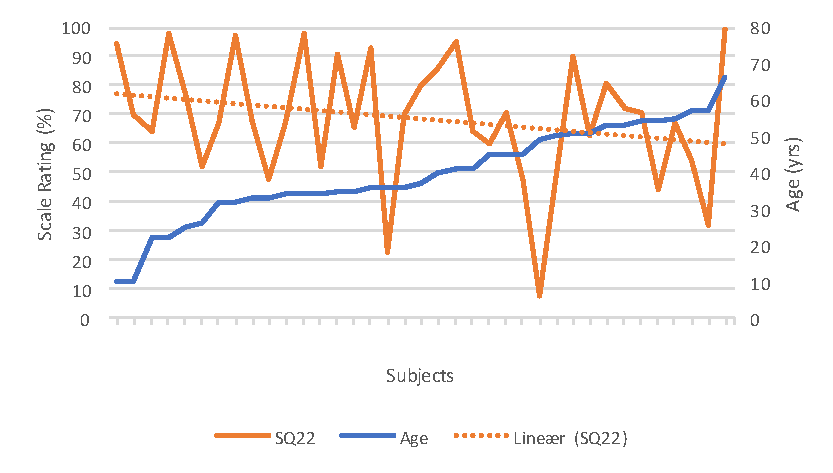
\includegraphics[width=\textwidth]{Figure/DatabehandlingSkalaer/Demografi/AgeSQ22}
\caption{Sammenhæng mellem hvad testpersonerne angiver (\%) på skalaen til SQ22: \textit{Hvad synes du om robotten?}, i forhold til \textit{sjov}, og deres alder. Denne graf bygger på 37 besvarelser, da der manglede seks.}
\label{fig:AgeSQ22}
\end{figure}
\noindent
%
Udover at analysere hvordan robottens højde påvirker testpersonernes respons vælges det, at analysere højdeforskellen mellem robot og testperson. Sammenholdes SQ4, vedrørende robottens bevægelser, med højdeforskellen forekommer der en lille positiv korrelation, jævnfør \autoref{fig:HeightRatioSQ4}, hvor det tyder på, at desto større højdeforskellen er mellem robot og testperson, desto mere vilde opleves robottens bevægelser. Dog skal der tages forbehold for, at der forekommer relativt stor variation mellem testpersonernes besvarelser. 
%
\begin{figure}[H]
\centering
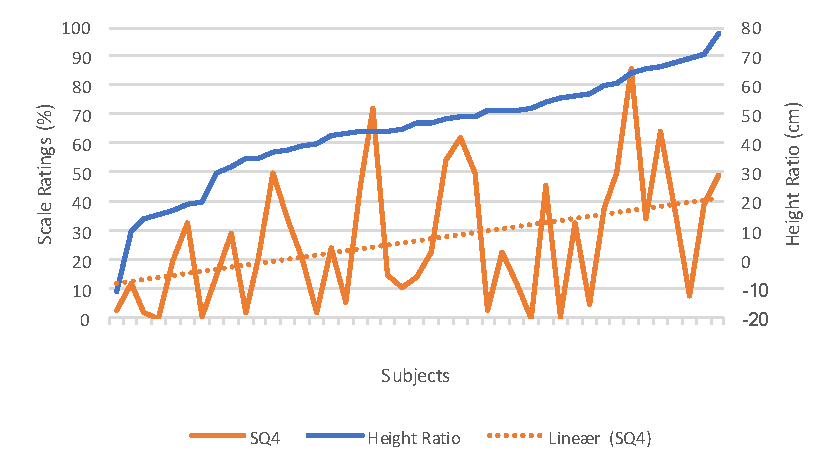
\includegraphics[width=\textwidth]{Figure/DatabehandlingSkalaer/Demografi/HeightRatioSQ4}
\caption{Sammenhæng mellem hvad testpersonerne angiver (\%) på skalaen til SQ4: \textit{Hvordan oplevede du robottens bevægelser?}, og højdeforskellen. Denne graf bygger på samtlige besvarelser.}
\label{fig:HeightRatioSQ4}
\end{figure}
\noindent
%
Der forekommer en positiv korrelation mellem højdeforskellen og SQ6, vedrørende robottens hastighed, jævnfør \autoref{fig:HeightRatioSQ6}. Det tyder på, at desto større højdeforskellen er, desto hurtigere opleves robotten. Dette hænger formentlig sammen med, at når robotten er på sit laveste (118 cm), så kører den hurtigere end når den eksempelvis er på sit højeste (151 cm). Sammenholdes det med en stor højdeforskel kan det formentlig virke som om, at robotten er endnu hurtigere. 
%
\begin{figure}[H]
\centering
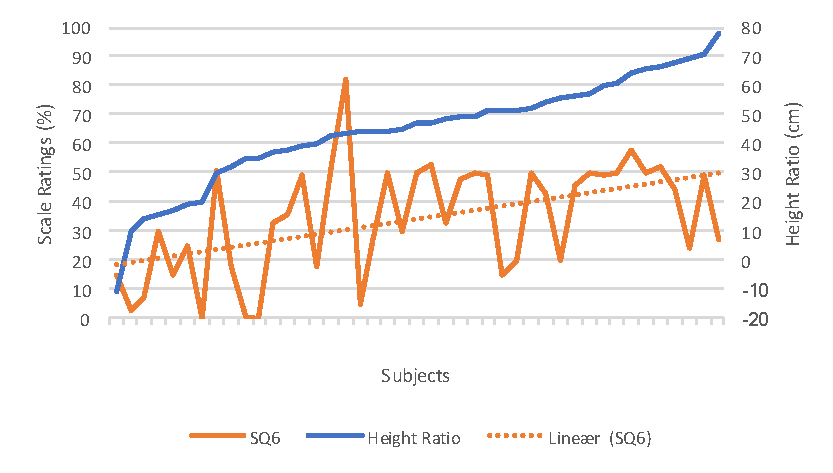
\includegraphics[width=\textwidth]{Figure/DatabehandlingSkalaer/Demografi/HeightRatioSQ6}
\caption{Sammenhæng mellem hvad testpersonerne angiver (\%) på skalaen til SQ6: \textit{Jeg synes, at robottens hastighed er...}, og højdeforskellen. Denne graf bygger på samtlige besvarelser.}
\label{fig:HeightRatioSQ6}
\end{figure}
\noindent
%
Sammenholdes højdeforskellen med SQ19, vedrørende hvor sød robotten opleves, forekommer der en positiv korrelation, jævnfør \autoref{fig:HeightRatioSQ19}. Denne korrelation indikerer, at desto større højdeforskellen er, desto sødere opleves robotten. 
%
\begin{figure}[H]
\centering
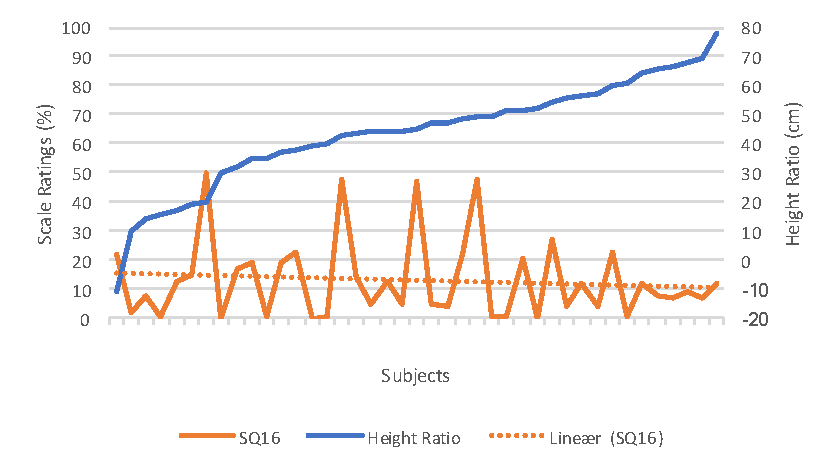
\includegraphics[width=\textwidth]{Figure/DatabehandlingSkalaer/Demografi/HeightRatioSQ19}
\caption{Sammenhæng mellem hvad testpersonerne angiver (\%) på skalaen til SQ19: \textit{Hvad synes du om robotten?}, i forhold til \textit{sød}, og højdeforskellen. Denne graf bygger på 41 besvarelser, da der manglede to.}
\label{fig:HeightRatioSQ19}
\end{figure}
\noindent
%
Baseret på \autoref{fig:BarPlotTechFrekvens} fremgår det, at størstedelen af testpersonerne er glade for teknologi, hvor 16 ud af 43 testpersoner har angivet en respons mellem 91 \% og 100 \%. Derudover tyder det på, at mændende (M=76.85, SD=22) er mere glad for teknologi end kvinderne (M=67.3, SD=30.2), fælles for begge køn er dog, at standardafvigelsen er meget høj, hvorfor det ikke endeligt kan fastslås. 
%
\begin{figure}[H]
\centering
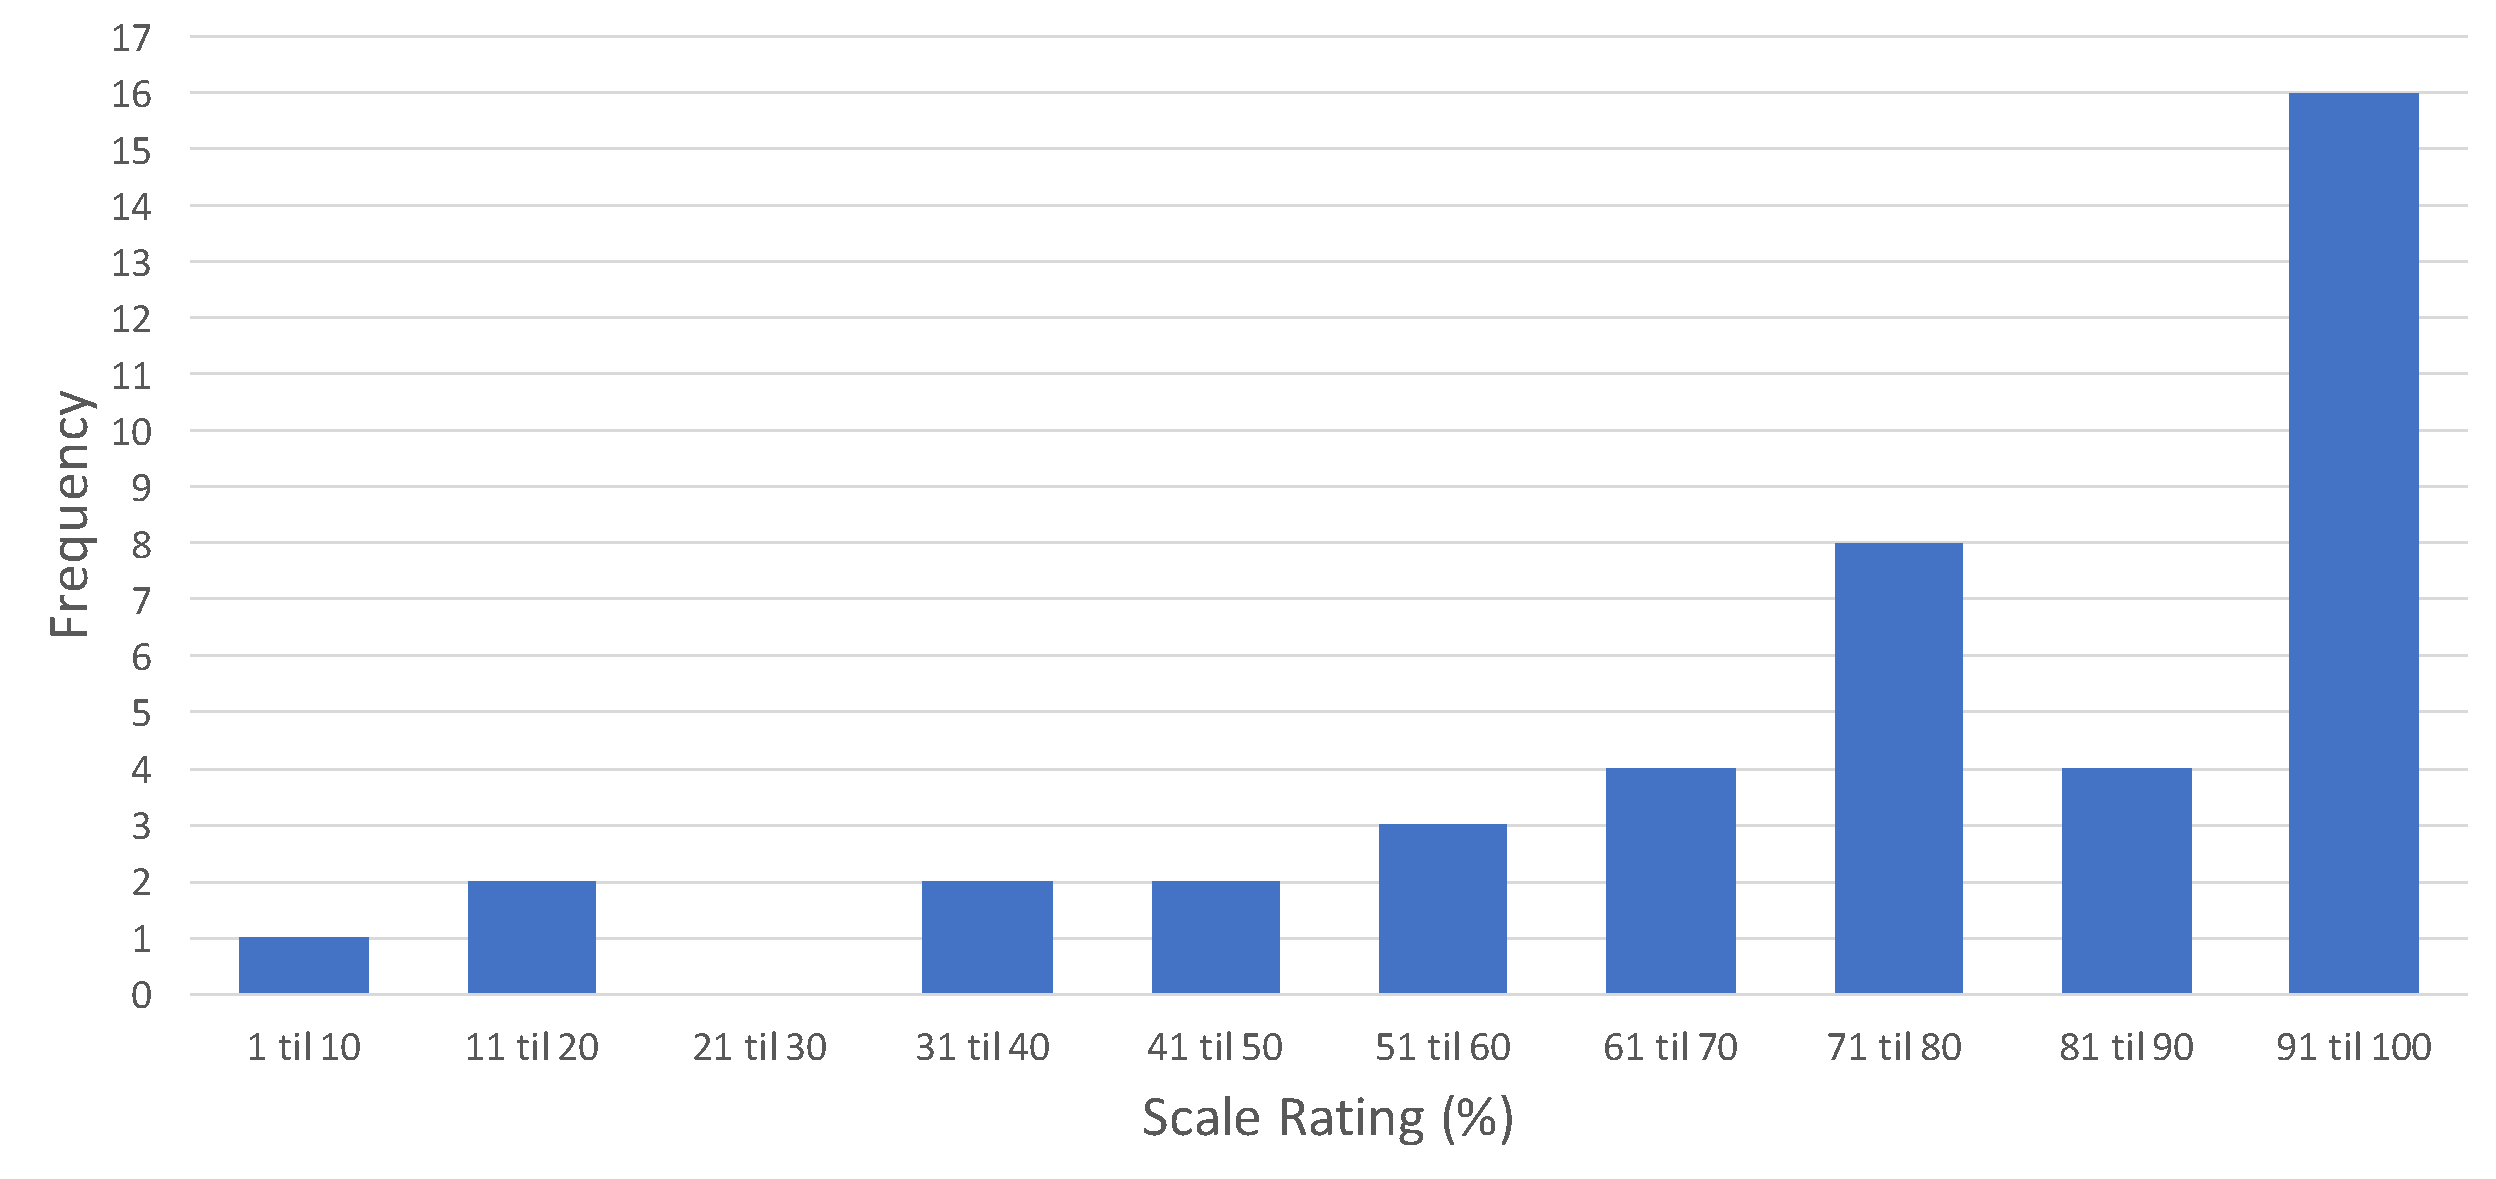
\includegraphics[width = \textwidth]{Figure/DatabehandlingSkalaer/DataPresentation/HistogramTek} 
\caption{Histogram over besvarelserne (\%) til skala spørgsmålet: \textit{Hvor glad er du for teknologi?}, som indgår i demografien.}
\label{fig:HistogramTek}
\end{figure}
\noindent
%
I forhold til hvilken indflydelse det har, at testpersonerne er glade for teknologi eller ej, tyder det ikke på at der er forekommet nogle korrelationer i forhold til specifikke skalaer. Selvom der ikke forekommer en korrelation mellem hvor godt skærmen reagerede og hvor glad testpersonerne var for teknologi, så er det ikke utænkeligt at de to parametre måske har en indflydelse på hinanden. At det ikke vides skyldes hovedsageligt at det ikke har været muligt at kontrollere hvordan skærmen reagerede, hvorfor det kun er deres subjektive vurdering af det. Den vurdering kan være præget af hvor glad testpersonerne er for teknologi, hvor nogle formentlig vil være mere overbærerne når skærmen ikke reagerede første gang og andre vil blive irriteret eller frustreret over det. Det kan både gøre sige gældende for testpersonerne, som er meget glad for teknologi og for testpersoner, som ikke er. 
